\documentclass[aspectratio=169,10pt]{beamer}

\usetheme{Madrid}
\usecolortheme{dolphin}
\usepackage[T1]{fontenc}
\usepackage[utf8]{inputenc}
\usepackage{amsmath,amssymb,booktabs}

\definecolor{courseblue}{RGB}{28,73,122}
\definecolor{accent}{RGB}{176,78,36}
\setbeamercolor{structure}{fg=courseblue}
\setbeamercolor{alerted text}{fg=accent}
\setbeamertemplate{navigation symbols}{}
\setbeamertemplate{footline}[frame number]

\newcommand{\Istar}{I^{*}}
\newcommand{\Ktilde}{\widetilde K}
\newcommand{\Itilde}{\widetilde I}
\newcommand{\sigHat}{\widehat\sigma}

\title{The Race between Man and Machine}
\subtitle{Automation, new tasks, wages, and factor shares}
\author{Repository 6 --- Artificial Intelligence and Economic Modeling}
\institute{Acemoglu \& Restrepo (AER, 2018)}
\date{}

\begin{document}

\begin{frame}
  \titlepage
  \vspace{-1em}
  \begin{center}
    \small Economic analysis: published AER 108(6), 1488--1542\\
    Lean source: NBER Working Paper 22252, revised June 2017
  \end{center}
\end{frame}

\begin{frame}{Research question and core answer}
\begin{block}{Question}
Does automation necessarily reduce wages and the labor share?
\end{block}
\begin{itemize}
  \item Automation must first change \emph{effective} task allocation:
        $I$ is technological capability, while $\Istar$ is equilibrium automation.
  \item If automation reallocates tasks, the labor share falls through
        \alert{displacement}.
  \item The wage is conditional because displacement competes with a positive
        \alert{productivity effect}.
  \item New labor-intensive tasks create a \alert{reinstatement effect}.
\end{itemize}
\begin{alertblock}{Bottom line}
The labor-share effect is one-sided under the relevant static conditions; the
wage effect is not.
\end{alertblock}
\end{frame}

\begin{frame}{Continuum of tasks and final output}
Tasks are indexed on a continuum:
\[
  i\in[N-1,N].
\]
Each task produces an intermediate $y(i)$, and the final good aggregates all
tasks with constant elasticity:
\[
  Y=\left(\int_{N-1}^{N} y(i)^{\frac{\sigma-1}{\sigma}}\,di
  \right)^{\frac{\sigma}{\sigma-1}}.
\]
\begin{itemize}
  \item A task is an activity required to produce final output.
  \item The interval has unit measure; $N$ locates the frontier of task content.
  \item Task allocation is therefore an endogenous margin of aggregate production.
\end{itemize}
\end{frame}

\begin{frame}{Task technologies and comparative advantage}
For tasks that machines can perform ($i\le I$), either factor may be used:
\[
  y(i)=\bigl[k(i)+\gamma(i)l(i)\bigr]^{1-\eta}q(i)^{\eta}.
\]
For nonautomatable tasks ($i>I$), labor is required:
\[
  y(i)=\bigl[\gamma(i)l(i)\bigr]^{1-\eta}q(i)^{\eta}.
\]
\begin{itemize}
  \item $\gamma(i)$ is increasing: labor has comparative advantage in
        higher-index tasks.
  \item Effective factor costs are $R$ for capital and $W/\gamma(i)$ for labor.
  \item An automatable task uses capital when $R<W/\gamma(i)$.
\end{itemize}
\end{frame}

\begin{frame}{Technological frontier $I$ versus effective frontier $\Istar$}
Define the cost frontier by
\[
  \frac{W}{R}=\gamma(\Itilde).
\]
Equilibrium automation is
\[
  \boxed{\Istar=\min\{I,\Itilde\}}.
\]
\begin{columns}[T]
\column{0.48\textwidth}
\begin{block}{Technology constrained}
$I<\Itilde$, hence $\Istar=I$. A rise in $I$ moves the effective frontier and
reassigns the marginal task to capital.
\end{block}
\column{0.48\textwidth}
\begin{block}{Cost constrained}
$\Itilde<I$, hence $\Istar=\Itilde$. A rise in $I$ expands feasibility but does
not change actual task assignment.
\end{block}
\end{columns}
\vspace{0.4em}
\alert{Technological possibility is not the same as effective automation.}
\end{frame}

\begin{frame}{Displacement effect}
Consider a static automation-only change with fixed $K$:
\[
  dI>0,\qquad dN=0,\qquad \Istar=I<\Itilde.
\]
\begin{enumerate}
  \item Newly automatable marginal tasks move from labor to capital.
  \item Labor is compressed into a smaller set of tasks.
  \item Diminishing returns within the remaining labor tasks reduce relative
        labor demand.
\end{enumerate}
Proposition 2 gives
\[
  \frac{d\ln(W/R)}{dI}
  =-\frac{\Lambda_I}{\sigHat+\varepsilon_L}<0.
\]
Thus effective automation lowers $W/R$, the labor share, and employment under
the paper's labor-supply specification.
\end{frame}

\begin{frame}{Productivity effect and the wage}
Automation also replaces expensive effective labor with cheaper capital:
\[
 d\ln Y\big|_{K,L}>0.
\]
For the technology-constrained allocation, Proposition 3 decomposes the wage:
\[
d\ln W=d\ln Y\big|_{K,L}
+(1-s_L)\left[
\frac{\Lambda_N}{\sigHat+\varepsilon_L}\,dN
-\frac{\Lambda_I}{\sigHat+\varepsilon_L}\,dI
\right].
\]
With $dN=0$:
\[
\underbrace{d\ln W}_{\text{ambiguous}}
=\underbrace{d\ln Y\big|_{K,L}}_{\text{productivity }(+)}
-\underbrace{(1-s_L)\frac{\Lambda_I}{\sigHat+\varepsilon_L}\,dI}
_{\text{displacement }(-)}.
\]
Output can rise while the wage falls.
\end{frame}

\begin{frame}{When can automation raise the wage?}
Under AER Assumptions 1--3, Proposition 3 establishes a finite threshold
$\Ktilde$:
\[
  K>\Ktilde \ \Longrightarrow\ \frac{d\ln W}{dI}>0,
  \qquad
  K<\Ktilde \ \Longrightarrow\ \frac{d\ln W}{dI}<0.
\]
\begin{itemize}
  \item At low $K$, the cost-saving gap at the marginal task is small:
        displacement dominates.
  \item At high $K$, capital is abundant and the productivity gain can dominate.
  \item This concerns the \emph{absolute wage}; it does not reverse the fall in
        $W/R$ or the labor share.
\end{itemize}
\begin{alertblock}{Source discipline}
Published AER version, Proposition 3, pp.~1501--1503.
\end{alertblock}
\end{frame}

\begin{frame}{Labor share and employment}
Why can the wage rise while the labor share falls?
\[
  s_L=\frac{WL}{RK+WL},
  \qquad
  \frac{d\ln(W/R)}{dI}<0.
\]
\begin{itemize}
  \item Productivity can increase the level of $W$.
  \item Displacement changes relative factor demand in favor of capital.
  \item Hence $W$ and $W/R$ need not move together.
  \item Under equation (4)'s labor-supply preferences, automation raises output
        per worker more than the wage, so employment falls.
\end{itemize}
The capital share rises as the complementary net-output factor share.
\end{frame}

\begin{frame}{New tasks and reinstatement}
A higher $N$ introduces a new high-index task where labor has comparative
advantage. Under Assumption 3,
\[
  R>\frac{W}{\gamma(N)},
\]
so the new task is adopted with labor.
\begin{center}
\begin{tabular}{lccccc}
\toprule
Change & Output & Wage & Employment & Labor share & $W/R$\\
\midrule
Higher $N$ & $+$ & $+$ & $+$ & $+$ & $+$\\
\bottomrule
\end{tabular}
\end{center}
This is \alert{reinstatement}: labor returns to a wider range of activities. It
is not merely more productivity; it changes the task content of production in
labor's favor.
\end{frame}

\begin{frame}{Capital adjustment and endogenous technology}
\begin{block}{Long-run capital adjustment: Proposition 5}
On the relevant interior balanced-growth path,
\[
  R=\rho+\delta+\theta g.
\]
Capital adjustment passes productivity gains toward the relatively inelastic
factor. Long-run automation raises the wage but still lowers employment and the
labor share.
\end{block}
\begin{block}{Direction of innovation: Proposition 6 and Corollary 2}
A temporary automation imbalance can make further automation less attractive
and new-task creation more attractive. A permanent shift toward automation
instead leads to a new BGP with lower task content $n=N-I$, employment, and
labor share.
\end{block}
\end{frame}

\begin{frame}{Does automation necessarily reduce wages and labor share?}
\small
\begin{center}
\begin{tabular}{p{0.29\textwidth}p{0.28\textwidth}p{0.32\textwidth}}
\toprule
Experiment & Wage & Labor share\\
\midrule
$I$ rises but $\Istar$ does not & No marginal effect & No marginal effect\\
Effective automation, fixed $K$ & Conditional on productivity versus displacement
& Falls\\
Effective automation, $K$ adjusts on BGP & Rises under Proposition 5 conditions
& Falls\\
New tasks & Rises & Rises\\
\bottomrule
\end{tabular}
\end{center}
\begin{alertblock}{Rigorous answer}
No. Effective automation reduces the labor share under the relevant conditions,
but its wage effect depends on productivity, displacement, the capital stock,
and the adjustment horizon.
\end{alertblock}
\end{frame}

\begin{frame}{Where I did not believe the AI}
\begin{description}
  \item[AI initially wrote] AER equation (5) as effective task cost divided by
        $1-\eta$.
  \item[Why doubt it?] That expression did not match the task technology or the
        displayed source equation.
  \item[AER says]
  \[
    p(i)=\min\{R,W/\gamma(i)\}^{\,1-\eta}
    \quad\text{for } i\le I.
  \]
  \item[Correct interpretation] The positive power preserves the cost ranking,
        so the allocation frontier is unchanged, but division would give wrong
        task-price levels.
\end{description}
\small Source: published AER, equation (5), p.~1496. This was a real
transcription error, not a manufactured disagreement.
\end{frame}

\begin{frame}{Hand derivation: wage sign under automation}
\begin{center}
  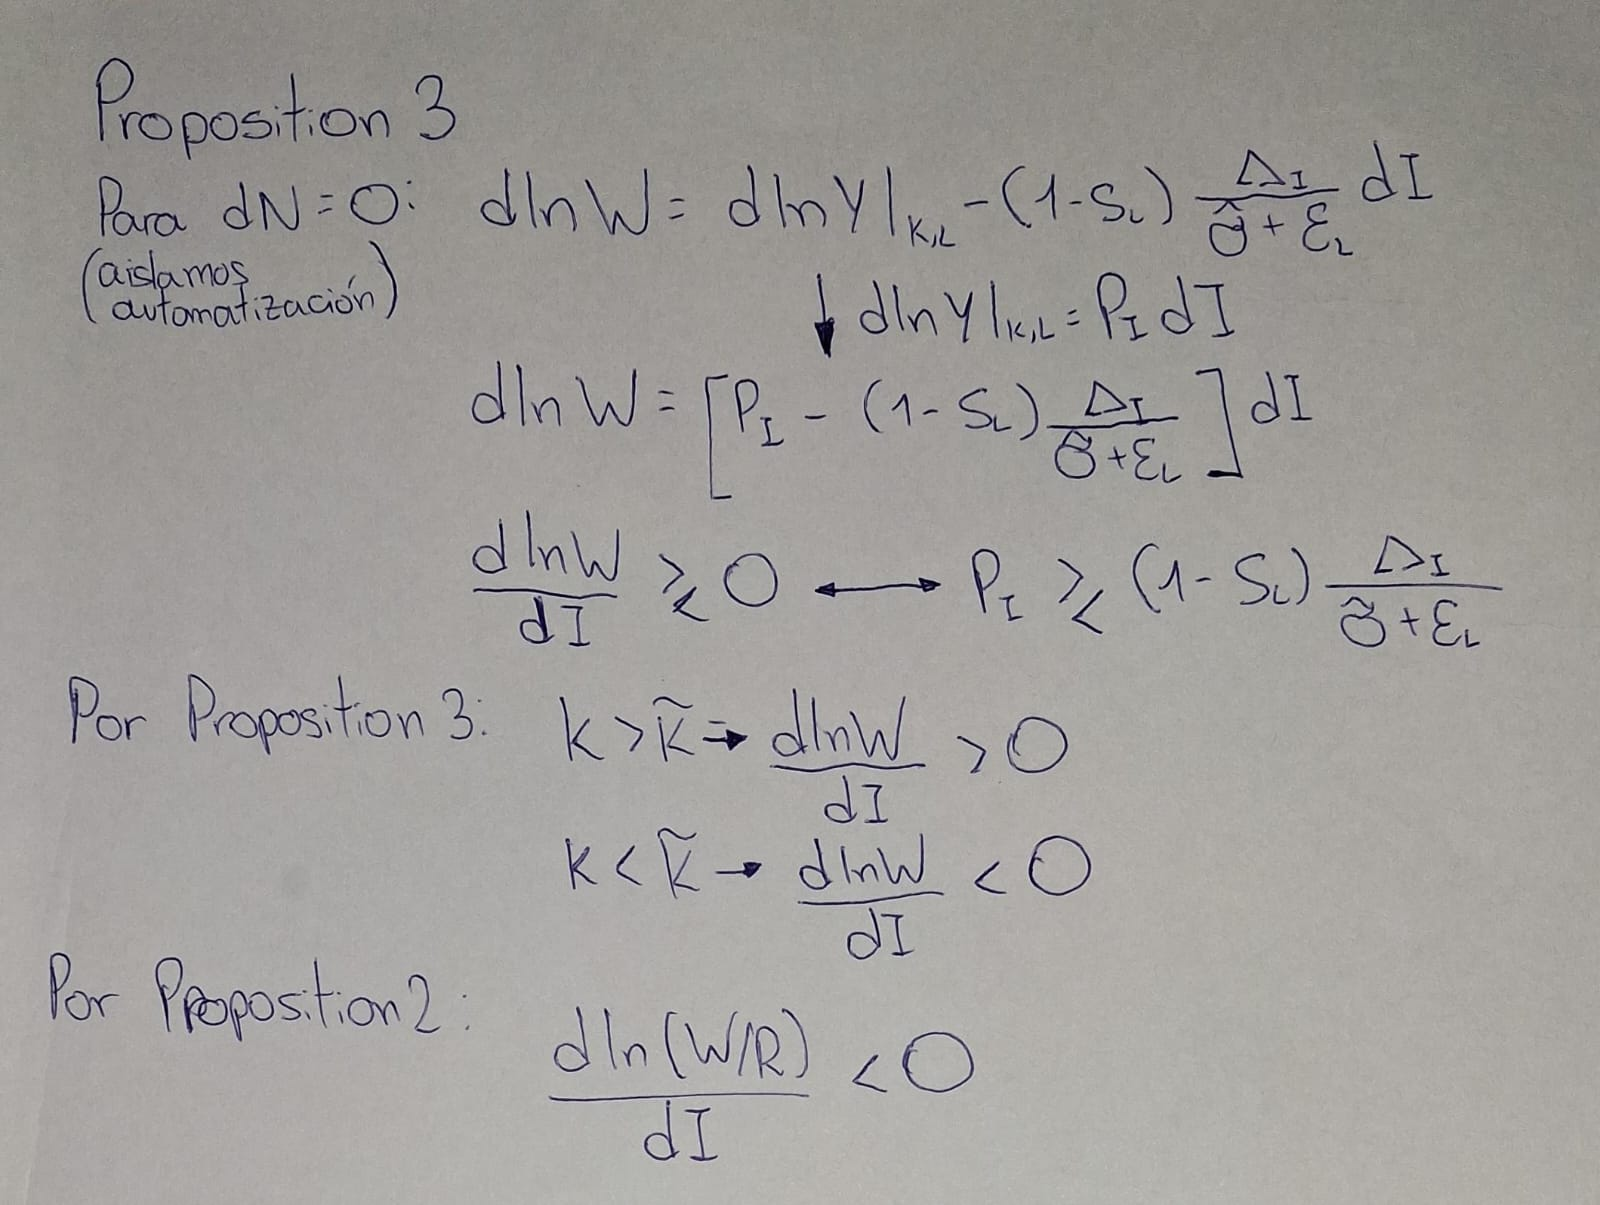
\includegraphics[height=0.82\textheight,keepaspectratio]{hand/derivation.jpeg}

  \vspace{0.2em}
  \scriptsize Real handwritten derivation: Proposition 3 wage threshold and
  Proposition 2 relative-factor-price result.
\end{center}
\end{frame}

\begin{frame}{Lean formalization: the narrow claim}
\small
\begin{block}{Paper source}
NBER Working Paper 22252, revised June 2017, Section 2.2, p.~8, equation (6)
and the threshold discussion immediately following it.
\end{block}
\[
  \frac{w}{r}=\gamma(c),\qquad
  e=\min\{a,c\},\qquad i<e.
\]
Lean proves the implication
\[
 i<\min\{a,c\}\quad\Longrightarrow\quad
 i\le a\ \land\ r<\frac{w}{\gamma(i)}.
\]
\begin{center}
\begin{tabular}{ll}
\toprule
Lean symbol & Economic meaning\\
\midrule
$a$ / \texttt{automationThreshold} & technological frontier\\
$c$ / \texttt{costThreshold} & cost frontier\\
$i$ & task index\\
$w,r,\gamma$ & wage, rental rate, labor productivity\\
\bottomrule
\end{tabular}
\end{center}
\end{frame}

\begin{frame}[fragile]{Lean proof and scope}
\scriptsize
\begin{columns}[T]
\column{0.53\textwidth}
\begin{block}{Core proof logic (identifiers romanized for the slide)}
\begin{verbatim}
have hiCost : i < costThreshold :=
  lt_of_lt_of_le hi (min_le_right _ _)
have hgammaLt : gamma i < w / r := by
  rw [hthreshold]
  exact hgamma hiCost
have hmul : gamma i * r < w :=
  (lt_div_iff0 hr).mp hgammaLt
apply (lt_div_iff0 (hgammaPos i)).mpr
simpa [mul_comm] using hmul
\end{verbatim}
\end{block}
\column{0.43\textwidth}
\textbf{Assumptions}
\begin{itemize}
  \item $\gamma$ strictly increasing and positive;
  \item $w>0$, $r>0$;
  \item $w/r=\gamma(c)$;
  \item $i<\min\{a,c\}$.
\end{itemize}
\textbf{Verified:} a task below both frontiers is feasible for capital and
capital is strictly cheaper.

\textbf{Not verified:} a full proposition, equilibrium, wage effects, shares,
dynamics, or balanced growth.
\end{columns}
\vspace{0.3em}
\begin{alertblock}{Actual result}
Focused build passed; \texttt{paper\_contribution.py check
AR18RaceManMachine --fast} passed. Semantic closeout remains pending in the
preserved audit scaffolding.
\end{alertblock}
\end{frame}

\begin{frame}{Conclusion}
\begin{enumerate}
  \item Only a change in $\Istar$, not capability $I$ alone, reallocates tasks.
  \item Effective automation creates displacement and productivity together.
  \item The labor share falls, but the wage can rise or fall at fixed capital;
        $\Ktilde$ separates the cases.
  \item New labor-intensive tasks reinstate labor and work in the opposite
        direction.
  \item Lean verifies one source-connected threshold implication---useful, but
        deliberately much narrower than the paper's economic propositions.
\end{enumerate}
\begin{alertblock}{Answer}
Automation does not necessarily reduce both wages and the labor share.
\end{alertblock}
\end{frame}

\end{document}
